\chapter{Development and Testing}
\label{chap:implementation}

\section{Backend Implementation}
\label{sec:backend-impl}

The backend follows a layered structure in which routes delegate to controllers, controllers
delegate to services, and only services interact with the data models. Business logic is kept
out of route handlers so that it can be unit tested without an HTTP server.

Authorisation for video access is concentrated in a single service function. Every path that
exposes a video, whether the detail endpoint, the like and comment endpoints, or the playback
authorisation endpoint, calls that same function. This is a deliberate choice: duplicating the
permission check across endpoints is the most common way for an access control gap to appear,
because a later change updates one copy and not the others.

The upload flow validates metadata on the server before issuing a pre-signed URL. Client-side
validation alone is insufficient, since a user can call the API directly and obtain a URL for
an arbitrary file, effectively turning the project's storage bucket into free hosting for
unrelated content. The server therefore checks the declared MIME type against an allow-list of
video formats and rejects files exceeding two gigabytes.

Several protective measures were added at the HTTP layer. Security headers are applied through
Helmet. Cross-origin requests are restricted to an explicit allow-list rather than being
accepted from any origin, which is also a prerequisite for signed cookies to work, because the
CORS specification forbids credentials in combination with a wildcard origin. Authentication
endpoints are rate limited to ten attempts per fifteen minutes per address, which makes
password guessing impractical without affecting legitimate users. Finally, the process
validates its required environment variables at startup and refuses to start if the token
signing secret is missing, converting a dangerous runtime failure into an immediate and obvious
one.

\section{Transcoder Implementation}
\label{sec:transcoder-impl}

The transcoder is a Node.js worker packaged with FFmpeg in a Docker image built through a
multi-stage build. The base image went through two upgrades over the course of the project.
Node 18 was used initially but had to be abandoned because Mongoose 9 depends on the Web Crypto
API, which is not fully available in that version, causing the container to fail when connecting
to MongoDB Atlas. Node 20 was then adopted, and later replaced with \texttt{node:24-slim} once
Node 20 reached end-of-life on 30 April 2026 and stopped receiving security patches; Node 24 was
chosen over the newer Node 26 because it is the current Active LTS release, supported until April
2028, whereas Node 26 had not yet entered its LTS phase at the time of the upgrade. The Alpine
variant was avoided throughout because FFmpeg requires glibc.

The heartbeat mechanism described in Section~\ref{sec:pipeline-design} is, in effect, a lease in
the sense introduced by Burrows for the Chubby lock service \cite{burrows2006chubby}: a holder
retains a resource by periodically renewing it before a timeout expires, and Burrows already
identified the classical failure mode of that pattern: a lease can expire while its holder is
merely stalled rather than dead, so a second holder may be granted the same resource while the
first is still alive and will eventually act on it. A defect matching exactly this failure mode
surfaced during a literature-driven review of the pipeline's reliability guarantees, discussed
further in Section~\ref{sec:testing}: neither \texttt{updateVideoReady} nor
\texttt{updateVideoError} checked the video's current status before writing, so a duplicate job
triggered by an SQS redelivery could silently overwrite a successful result, and in the worst
case could revert an already-\texttt{READY} video back to \texttt{ERROR}. Both functions were
changed to a conditional \texttt{findOneAndUpdate} that only writes when the current status is
not already \texttt{READY}, and \texttt{processVideo} now checks the video's status before
downloading anything, so a duplicate delivery that arrives after the first job has already
finished is rejected immediately instead of re-downloading and re-transcoding the source.

A single FFmpeg invocation produces all three renditions, which is more efficient than three
separate invocations because the source is decoded only once. The command emits segments of six
seconds, generates the per-rendition playlists, and the worker then writes the master playlist
that lists the available bandwidths and resolutions. A thumbnail is extracted in a separate
pass.

Failure handling is deliberate. When FFmpeg exits with a non-zero status, the error propagates
to the top-level handler, which records the \texttt{ERROR} status in the database and, in
\texttt{worker} mode, does \emph{not} delete the SQS message: leaving it in flight allows the
visibility timeout to lapse so that the job is retried, and after the configured number of failed
attempts the message is moved to the dead letter queue where it can be inspected rather than lost.

As Section~\ref{sec:pipeline-design} establishes, however, the deployed system runs \texttt{batch}
mode, where the container holds no message to retain. The retry and dead-letter behaviour just
described therefore governs only the Lambda that submits jobs, not the transcoding itself, and the
recording of \texttt{ERROR} in the database is the sole part of this paragraph that applies to a
deployed transcoding failure. The gap this left, and its consequences for how such failures were
detected, is examined in Section~\ref{sec:challenges}.

\section{Infrastructure as Code}
\label{sec:iac}

The AWS environment is described by eleven Terraform modules, summarised in
Table~\ref{tab:terraform-modules}, and is instantiated separately for the development and
production environments.

\begin{table}[H]
\centering
\caption{Terraform modules and their responsibilities}
\label{tab:terraform-modules}
\small
\begin{tabularx}{\textwidth}{p{0.14\textwidth} X}
\toprule
\textbf{MODULE} & \textbf{RESPONSIBILITY} \\
\midrule
\texttt{s3}         & Raw and processed buckets, CORS configuration, Glacier lifecycle transition, event notification \\
\texttt{sqs}        & Transcode queue, dead letter queue with a redrive policy, queue access policy \\
\texttt{ecr}        & Container registry with image scanning on push and a lifecycle policy retaining recent images \\
\texttt{iam}        & Execution roles for AWS Batch, the ECS task, the transcoder task, and the Lambda submitter \\
\texttt{vpc}        & Virtual network, public subnets, internet gateway, security groups, S3 gateway endpoint \\
\texttt{secrets}    & AWS Secrets Manager entries for the database connection string and the token signing secret \\
\texttt{sns}        & Notification topics for transcode completion and dead letter queue alerts \\
\texttt{monitoring} & CloudWatch log groups, alarms, and dashboard \\
\texttt{batch}      & Fargate compute environment, job queue, and job definition \\
\texttt{lambda}     & Job submitter function and its SQS event source mapping \\
\texttt{cloudfront} & Distribution, Origin Access Control, cache policy, and the trusted key group used for signed cookies \\
\bottomrule
\end{tabularx}
\end{table}

Two configuration details are worth highlighting. The S3 lifecycle policy transitions raw
source files to Glacier after thirty days, since they are never read again once transcoding has
succeeded but must be retained in case a re-encode becomes necessary. The cache policy assigns
a long time-to-live to segments, which are immutable once produced, and a short one to
manifests, which may change if the set of renditions changes.

\section{CI/CD Pipeline and DevSecOps}
\label{sec:cicd}

Seven GitHub Actions workflows automate verification and deployment, as shown in
Figure~\ref{fig:cicd}.

% Xoay ngang: bảy hàng workflow, hàng dài nhất có năm bước nối tiếp. Đặt vừa
% bề rộng vùng chữ thì nhãn trong hình rơi xuống khoảng 4pt.
\begin{sidewaysfigure}
\centering
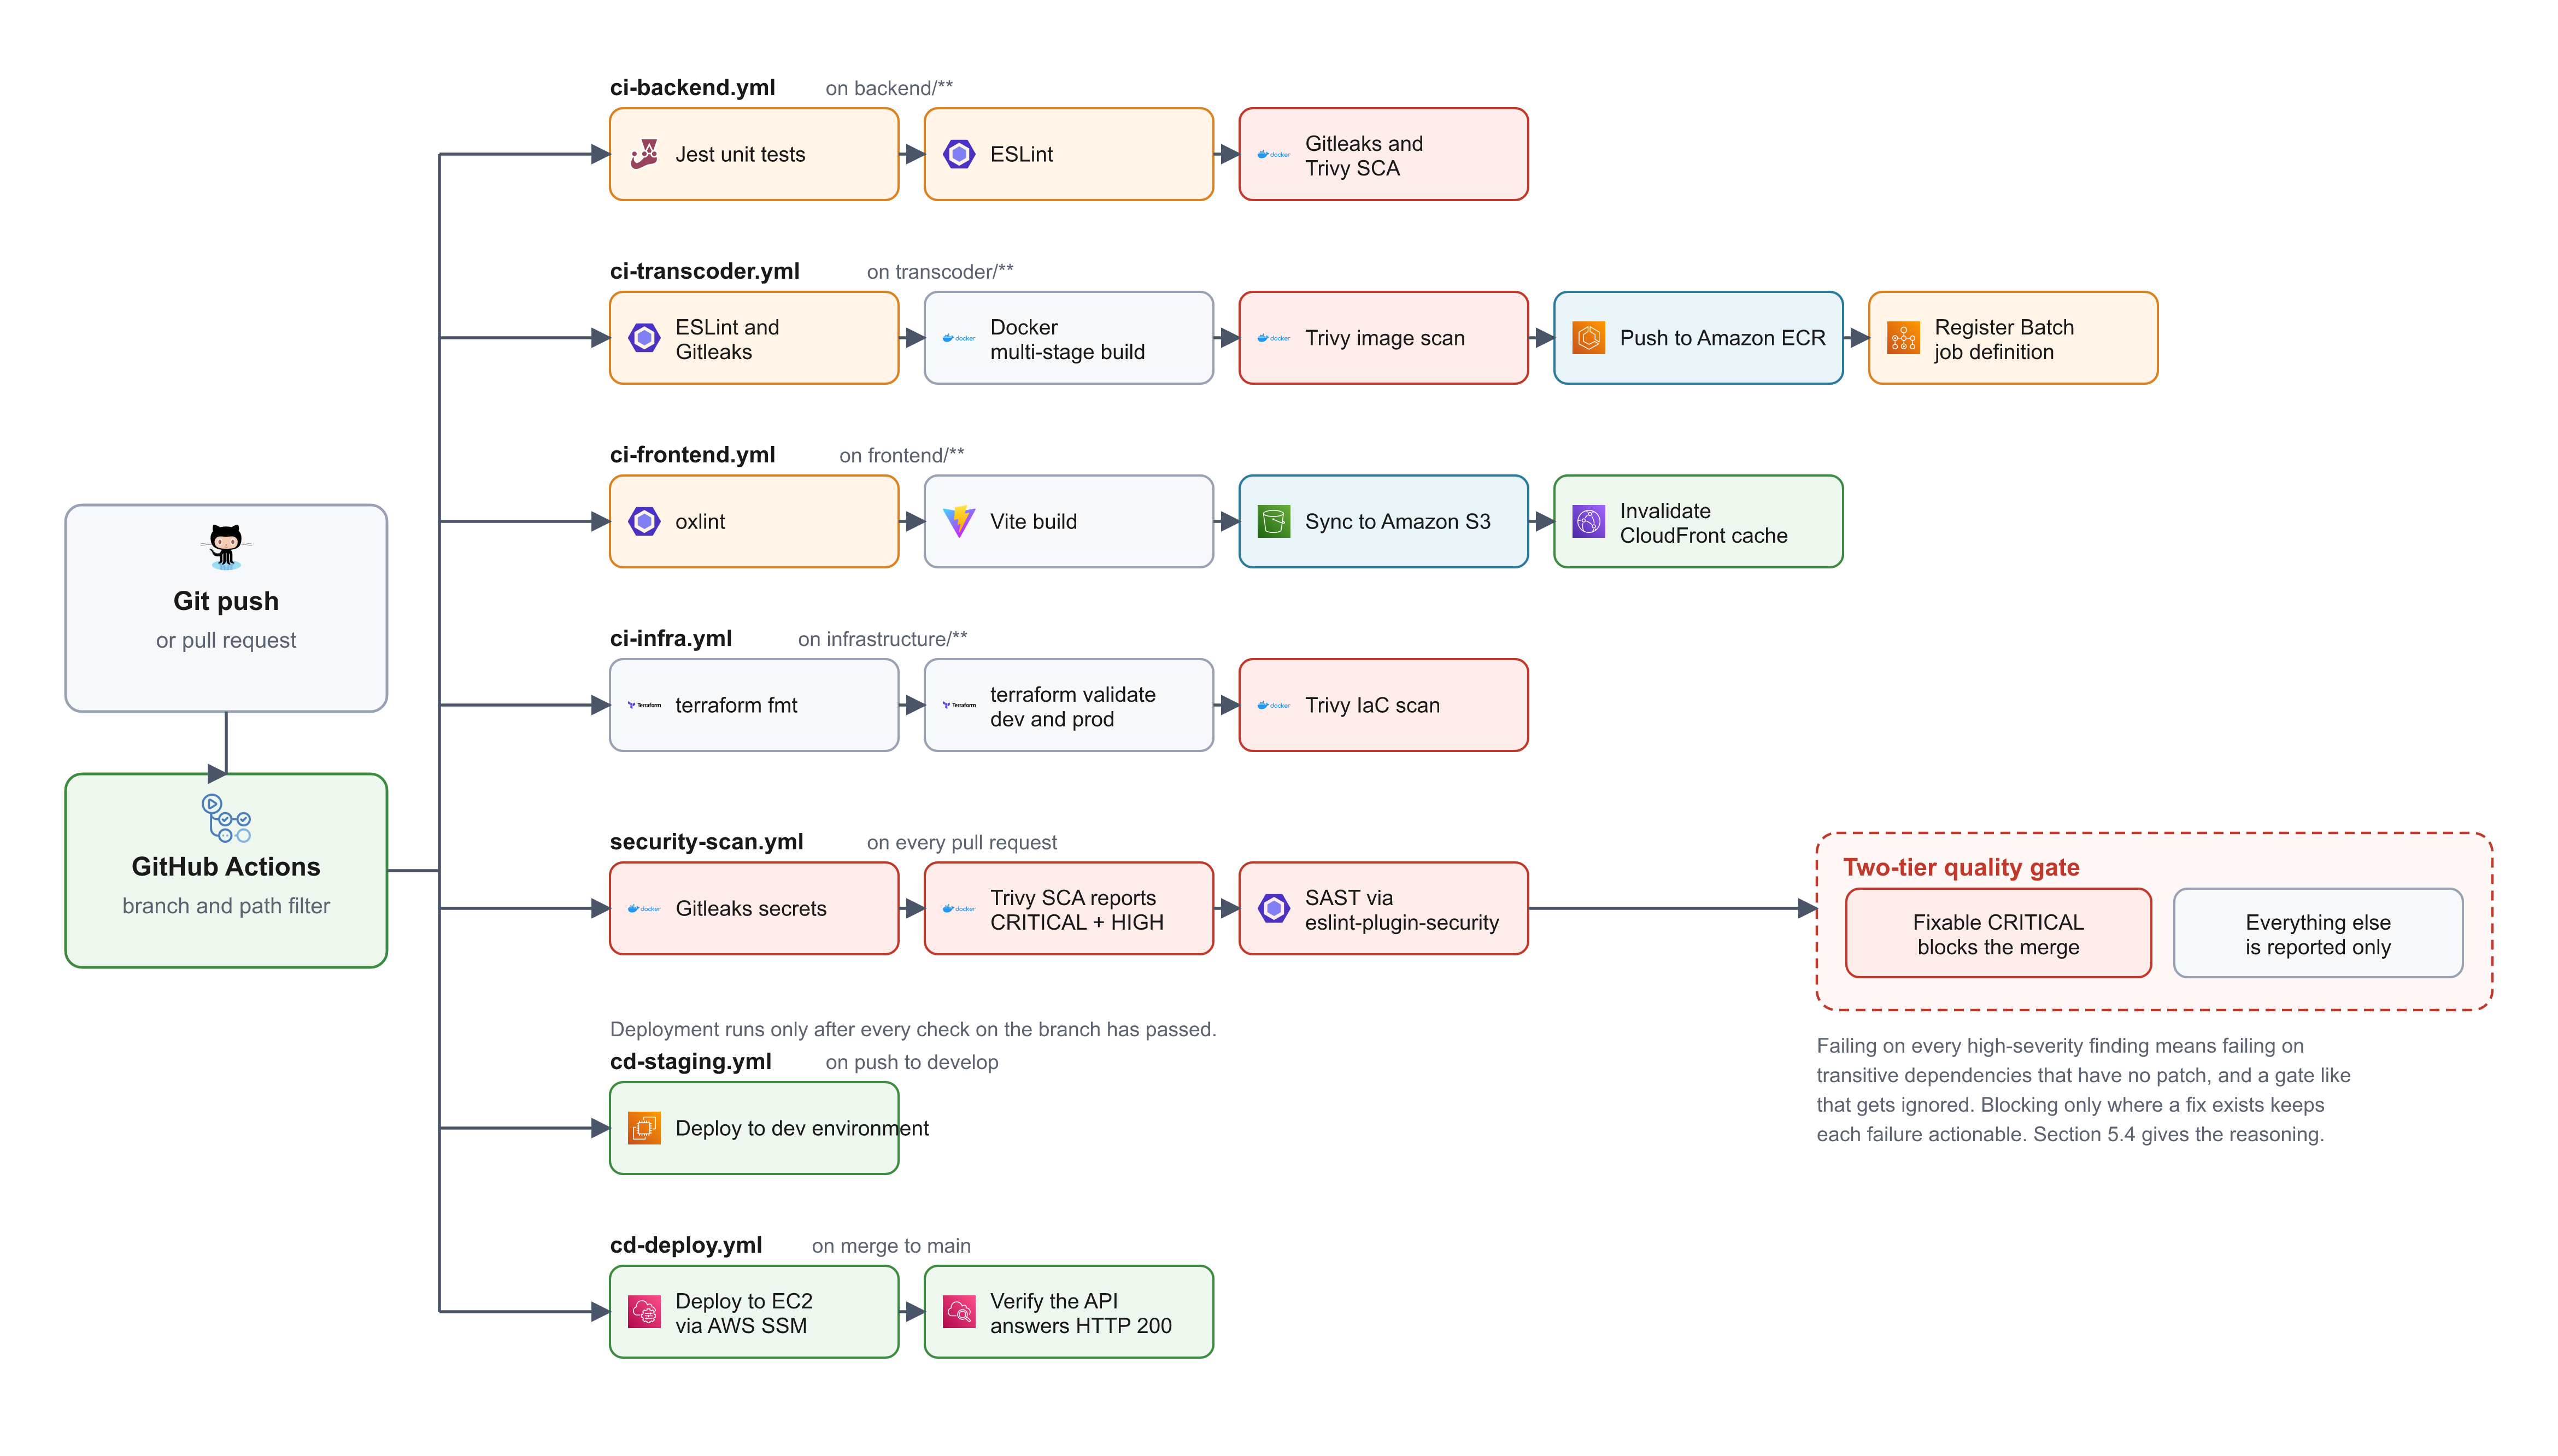
\includegraphics[width=\textheight]{images/03-cicd-pipeline.png}
\caption{\textit{The seven GitHub Actions workflows, the file paths that trigger each of them,
and the two-tier DevSecOps quality gate}}
\label{fig:cicd}
\end{sidewaysfigure}

The security gate is structured in two tiers, and the reason is practical. Scanning at the
combined critical and high severity levels and failing the build on any finding sounds
rigorous, but in practice most high-severity findings originate in transitive dependencies for
which no patch yet exists. A gate configured that way fails continuously for reasons the team
cannot act upon, and the predictable result is that developers begin ignoring it. The pipeline
therefore reports critical and high findings for visibility without blocking, and blocks only
on critical findings for which a fix is available. This keeps the gate meaningful, because a
failure now always corresponds to an action the team can actually take.

Static application security testing is performed with \texttt{eslint-plugin-security} rather
than SonarQube. The rule set detects patterns such as command execution built from user input,
regular expressions vulnerable to catastrophic backtracking, and cryptographically unsafe
random number generation. The choice avoids operating a separate analysis server while still
executing genuinely within the pipeline. Where a finding is a false positive, it is suppressed
with an inline annotation that documents why, which forces each suppression to be justified
rather than silently ignored.

Infrastructure code is validated in its own workflow, which checks formatting, initialises
without a remote backend so that no credentials are required, validates both environments, and
scans the configuration for insecure settings.

A later audit of the pipeline found a weakness in its own supply chain. All five workflows
referenced the vulnerability scanner as \texttt{aquasecurity/trivy-action@master}. A branch
reference resolves to whatever that repository's default branch contains at the moment a job runs,
so a change made there, including one made by someone who had compromised the action, would
execute inside this project's continuous integration, which holds AWS credentials. Every other
action in the pipeline was already pinned at least to a major version tag. The references are now
pinned to a release commit hash, with the version tag retained in a comment so that upgrades
remain deliberate and readable.

The same audit narrowed one permission. The Lambda that submits transcoding jobs held
\texttt{batch:SubmitJob} on \texttt{Resource: "*"}, which allowed it to submit to any job queue
in the account rather than the project's own. It is now scoped to the specific queue and job
definition. The scoping is expressed through the naming convention rather than by referencing the
Batch module's outputs, because the Batch module already depends on the IAM module for its roles
and referring back would introduce a dependency cycle; both modules carry a note recording the
coupling that this creates. The companion action \texttt{batch:DescribeJobs} keeps the wildcard,
because it accepts arbitrary job identifiers and AWS provides no resource-level control for it,
and the module records that reason in a comment so the wildcard is not mistaken for an oversight.

\section{Challenges During Development}
\label{sec:challenges}

Several difficulties arose between a design that was correct on paper and a system that behaved
correctly once deployed. Each is recorded here with the resolution adopted, because those
resolutions shaped parts of the final architecture.

\subsection{Provisioning Blocked by Account Policy}

The content protection scheme of Section~\ref{sec:content-protection} was implemented and covered
by unit tests well before it could be provisioned. Applying the Terraform configuration failed
with an access-denied error, because AWS requires manual account verification before a new account
may create CloudFront distributions, and the request filed to lift that restriction remained
pending with no bound on how long it might take. Until it was resolved the processed-content
bucket was reachable directly over the public internet, so the private visibility setting had no
effect at the storage layer.

The restriction was worked around by provisioning the distribution in a second AWS account not
subject to it. Terraform supports this without duplicating any module: the distribution, its
Origin Access Control, its cache and response-header policies, and its Signed Cookie trusted key
group were given an explicit \texttt{provider} argument pointing at the second account, while the
buckets, Batch, Lambda and the database connection remained in the original one. Only the bucket
policy could not move, since a bucket policy may be attached only by the account that owns the
bucket. This required no special handling, because an Origin Access Control policy is expressed as
a service principal together with an \texttt{AWS:SourceArn} condition naming the distribution, a
form that is indifferent to which account owns the ARN. With the distribution in place, the
temporary public bucket policy was removed and the bucket returned to being reachable only through
CloudFront.

\subsection{A Signed Cookie Policy That Matched Nothing}

Exercising Signed Cookies against the new distribution revealed that every request returned
\texttt{403 Forbidden}, for public and private videos alike. The function building the resource
pattern that a cookie authorises, \texttt{buildResourcePattern}, signed
\texttt{videos/*/\{videoId\}/*}, with a wildcard segment between the prefix and the identifier,
whereas the transcoder writes every rendition and the master playlist directly under
\texttt{videos/\{videoId\}/}. Each cookie was therefore well formed and correctly signed, and
authorised a resource that no viewer could request.

The existing unit test did not detect this because it compared the function's output against a
literal string copied from the function itself rather than against the transcoder's key layout, so
it could confirm only that the function had not changed. The pattern was corrected to
\texttt{videos/\{videoId\}/*} and the test rewritten to assert against the layout the transcoder
actually produces. Signed Cookies were then verified end to end against the deployed system: a
manifest request without a valid cookie is rejected at the edge, and the identical request
succeeds once the playback-authorisation endpoint has issued cookies for that video.

\subsection{Two Consequences of Gating Every Object}

Gating the whole bucket behind Signed Cookies also gated video thumbnails, which a catalogue
listing must render for many videos at once even though a cookie authorises exactly one. A
separate unsigned cache behaviour was carved out for the thumbnail path, since a thumbnail is not
the content the mechanism exists to protect.

Separately, the frontend's own CloudFront distribution, added because an Amazon S3 website
endpoint cannot return \texttt{200} for a single-page application's client-side routes on direct
navigation, had no cache-invalidation step in its deployment workflow, so a fix already synced to
the origin bucket continued to be served from the edge for hours afterwards. The workflow now
invalidates that distribution immediately after every deployment.

\subsection{Playback Across the Cookie Expiry Boundary}

Signed Cookies are valid for two hours, and the watch page requested them once when it mounted.
Crossing that boundary produced a \texttt{403} on the next segment, and the player's error handler
responded to any fatal network error by calling \texttt{startLoad()} with no attempt counter and
no delay, so an error that does not resolve on its own became an unbounded retry loop behind a
``reconnecting'' message that never changed.

Two properties of hls.js governed the fix. The library marks the first \texttt{403} as non-fatal
while it retries internally, so the handler must inspect the status code before filtering on the
fatal flag, or it discards the very error it exists to report. And \texttt{startLoad()} resumes
segment loading, whereas an expired cookie fails at the manifest, so recovery requires re-invoking
\texttt{loadSource()}. The handler now refreshes the cookies on a \texttt{403}, reloads the source,
and gives up after a bounded number of attempts with a message the viewer can act on.

\subsection{An Empty Secret That Stopped the Pipeline}

Every transcoding task began failing at \texttt{ResourceInitializationError} before its entrypoint
ran. The Terraform module for Secrets Manager created the entry holding the notification e-mail
password unconditionally but populated its value only when a password had been configured, so
leaving e-mail unconfigured produced a secret with no version carrying the \texttt{AWSCURRENT}
label. The Batch module decided whether to declare that secret in the job definition by testing
whether its ARN was non-empty, and the ARN of an empty secret is non-empty. The fix made the
secret itself conditional, so that the unconfigured state is internally consistent: no secret, an
empty ARN, and no declaration in the job definition.

The defect persisted longer than it should have because the only jobs submitted while it was live
belonged to the concurrency stress test, whose synthetic payloads were expected to fail. Checking
the cause recorded in \texttt{statusReason} rather than the terminal state alone would have
identified it immediately, and the alerting described next was changed to carry that field.

\subsection{Retry and Alerting on the Deployed Path}

Section~\ref{sec:pipeline-design} describes retry as delegated to SQS redelivery, which holds in
\texttt{worker} mode. On the deployed path the Lambda submitter deletes the message once the job
is submitted, so SQS no longer holds anything to redeliver, and the Batch job definition declared
no \texttt{retryStrategy}. Nothing retried a failed job at any layer, and a transient fault such
as a network error while downloading the source lost the video with no record beyond an
\texttt{ERROR} row.

Detection had the same shape. The alarm whose description read ``video transcoding failures
detected'' watched the depth of the dead letter queue, which receives a message only when the
Lambda fails to submit, so a job that fails after submission is invisible to it. The job
definition now declares three attempts, retrying infrastructure faults and exiting immediately
when the exit status indicates that FFmpeg rejected the content, together with a two-hour timeout
that bounds a process stalled on malformed input. Because AWS Batch publishes no CloudWatch metric
for failed jobs, an EventBridge rule matches job state transitions to \texttt{FAILED} and
publishes to the alert topic, with the notification carrying \texttt{statusReason}. The alarm
description was corrected to state what it genuinely covers.

\subsection{Monitoring the Service Rather Than the Server}

All four alarms watched the transcoding pipeline and none watched the backend API, which runs as a
single process on a single instance. The gap surfaced when assigning the backend a static address
moved its public IP while DNS still pointed at the released one, and the API returned
\texttt{522} for several minutes. Every infrastructure indicator stayed green, because nothing at
the infrastructure level was wrong.

A scheduled function now calls the public domain every five minutes along the same path a viewer
takes and publishes a metric that an alarm watches, with an instance status-check alarm alongside
it. A self-hosted check was chosen over a managed one on cost, since a managed health check on an
endpoint outside the provider costs roughly 1.75 USD per month against zero within the free tier,
and the trade-off it accepts, that checks originate from a single location, is recorded with the
implementation. The alarm's evaluation period is three times the check interval, so that each
window holds several datapoints and one late execution cannot open a gap that the missing-data
policy would read as a breach.

\subsection{Infrastructure Drift in the Instance Definition}

The AMI for the backend instance is resolved through a data source with
\texttt{most\_recent = true}, and the \texttt{ami} attribute forces replacement when it changes, so
every Ubuntu security release armed the next \texttt{terraform apply} to destroy and rebuild the
running server. What would have been lost is the state Terraform does not manage: the environment
file holding the database URI, signing key and mail credentials, the nginx configuration, the TLS
certificates, the process manager's state, and the public address that DNS points at. Changes to
the attribute are now ignored, which makes an image upgrade deliberate, and an Elastic IP keeps
the address stable across any rebuild that does occur.

\section{Testing}
\label{sec:testing}

The automated test suite comprises 117 tests across ten suites, summarised in
Table~\ref{tab:test-coverage}.

\begin{table}[H]
\centering
\caption{Automated test coverage by area}
\label{tab:test-coverage}
\small
\begin{tabularx}{\textwidth}{p{0.28\textwidth} p{0.10\textwidth} X}
\toprule
\textbf{SUITE} & \textbf{TESTS} & \textbf{FOCUS} \\
\midrule
\texttt{videoService}       & 11 & Upload initiation, ownership checks, deletion cascade \\
\texttt{s3Service}          & 2  & Key generation and pre-signed URL creation \\
\texttt{authService}        & 17 & Registration conflicts, login failures, token claims, password reset \\
\texttt{authMiddleware}     & 14 & Missing, malformed, forged, and expired tokens, and tokens issued before the account's last password change \\
\texttt{visibility}         & 21 & Privacy enforcement across every query path, view deduplication \\
\texttt{uploadValidation}   & 11 & HTTP-level validation of file type and size \\
\texttt{cloudfrontService}  & 24 & Cookie signing, policy scope, cookie attributes, and that revocation repeats the attributes used when issuing \\
\texttt{forgotPassword}     & 5  & That the response is identical whether or not the address has an account, including when e-mail delivery fails \\
\texttt{transcoder/dbHandler} & 6 & Conditional writes preventing duplicate-job overwrites \\
\path{transcoder/emailService} & 6 & READY/ERROR notification content and recipient targeting, and that raw failure detail is never exposed to the viewer \\
\bottomrule
\end{tabularx}
\end{table}

The visibility suite is the most important from a security standpoint, since it asserts that a
private video is absent from the public listing, returns a not-found response rather than a
forbidden one to non-owners, and remains accessible to its owner. Returning not-found is
deliberate: a forbidden response would confirm that a video with that identifier exists, which
leaks information.

The value of testing was demonstrated concretely during development of the signing service.
An initial implementation produced a canned policy, which the test suite immediately flagged
because the resulting cookie set contained an expiry field instead of a policy field. Since
canned policies do not support wildcard resources, that implementation would have failed for
every video once deployed. The defect was caught before any infrastructure was provisioned.

Testing caught a second defect in a similar way, this time surfaced not by writing a test first
but by a literature review of the reliability guarantees the pipeline was implicitly assuming
(Section~\ref{sec:transcoder-impl}). Once the conditional-write fix was implemented, six tests
were written to pin down the exact contract: a normal write succeeds when the video is not yet
\texttt{READY}; a write that loses the race to an earlier successful write is rejected and the
function returns the winning record rather than throwing; and a late failure from a duplicate job
can never revert an already-\texttt{READY} video to \texttt{ERROR}. As a falsifiability check, the
same six tests were run against the original, unconditional implementation: four of the six
failed, either because it never calls \texttt{findOneAndUpdate} at all or because it crashes
outright when handed a plain record with no \texttt{save} method, which is exactly the shape a
conditional read would have to return. The two that still passed were the not-found cases, which
neither version distinguishes from a duplicate write. The result confirms both that the new tests
are actually exercising the fixed code path and that the original implementation could not have
satisfied the contract by construction, not merely by accident of the test data chosen.
